\part{Entrega 1}

\begin{center}
    \href{https://github.com/LukasWolff2002/PROYECTO_1_MCOC_ENTREGA_1}{Ver repositorio GitHub.}
\end{center}

\setcounter{section}{0}

\section{Introducción}

\section{Marco Teórico}



\section{Desarollo}

\subsection{Caso 1}

\begin{figure}[H]
    \centering
    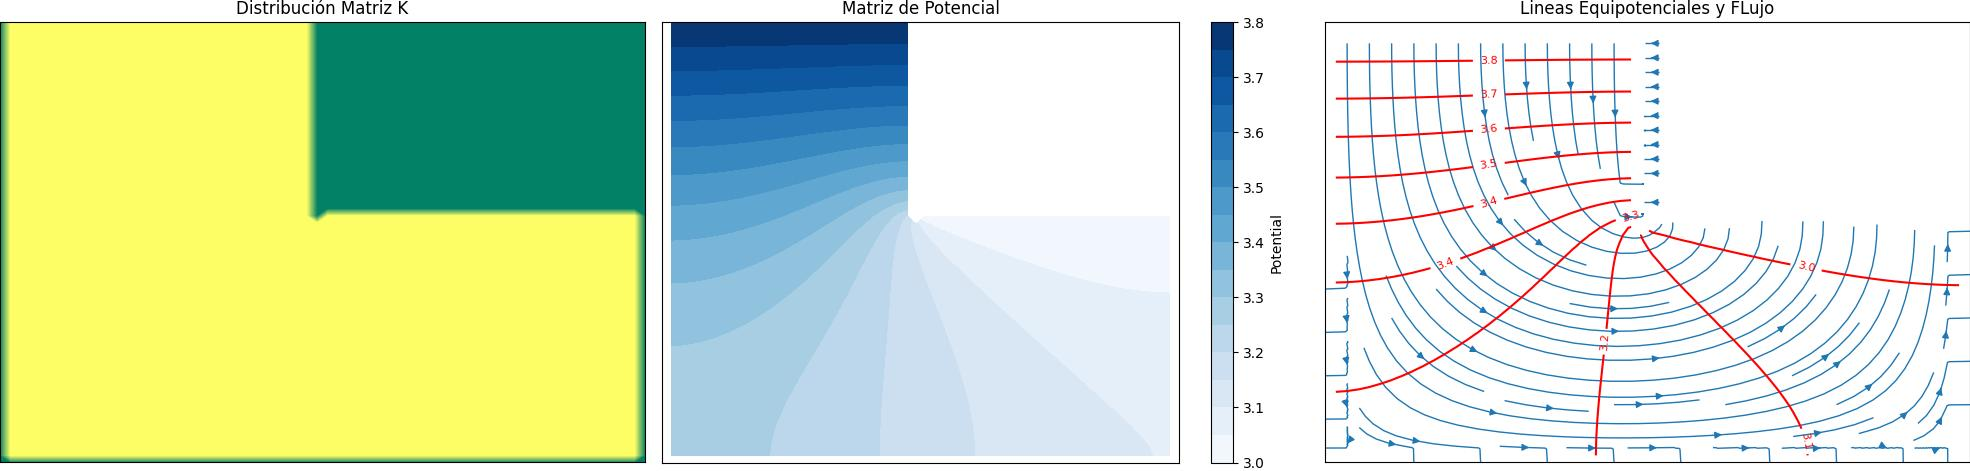
\includegraphics[width=1\textwidth]{GRAFICOS/laplace_caso_1.jpg}
    \caption{Gráfico de la función $f(x) = x^2$}
    \label{fig:caso_1}
\end{figure}

Se alcanzo la convergencia en la \textbf{iteracion 10588}
\\ \\
La velocidad de salida obtenida fue de \textbf{2.44e-05} m/s

\subsection{Caso 2}

\begin{figure}[H]
    \centering
    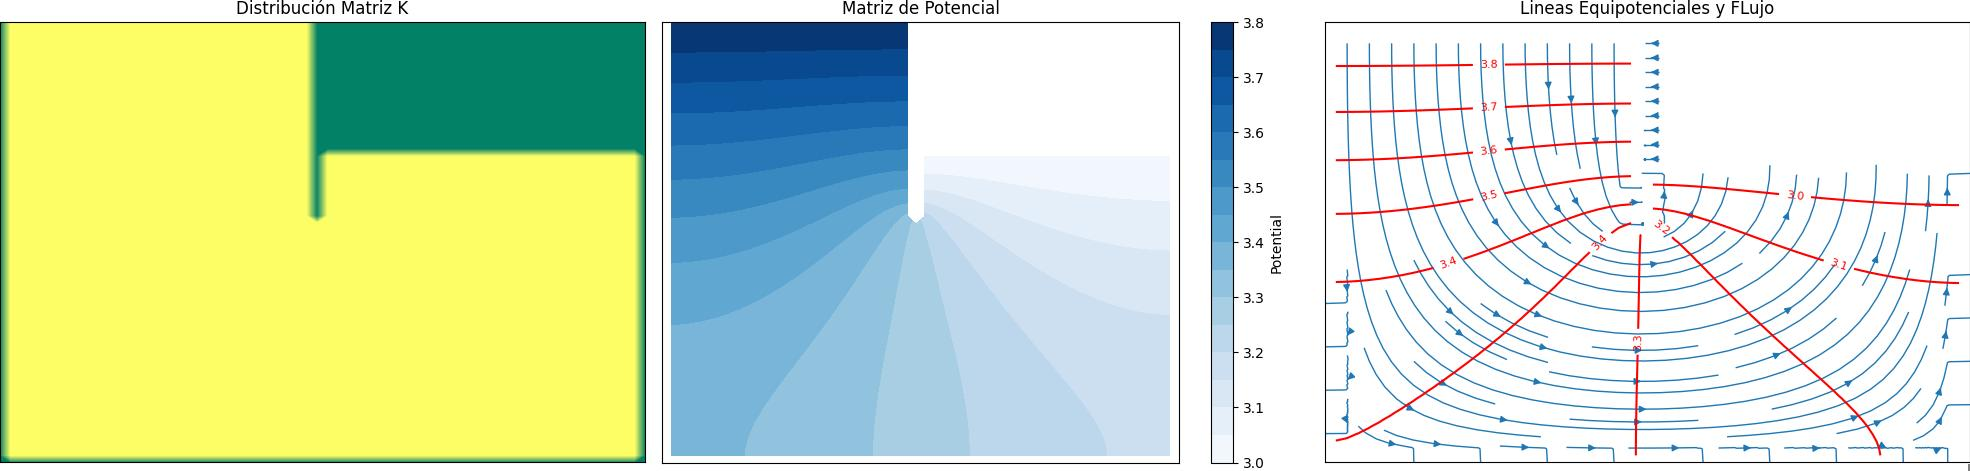
\includegraphics[width=1\textwidth]{GRAFICOS/laplace_caso_2.jpg}
    \caption{Gráfico de la función $f(x) = x^2$}
    \label{fig:caso_2}
\end{figure}

Se alcanzo la convergencia en la \textbf{iteracion 15651}
\\ \\
La velocidad de salida obtenida fue de \textbf{2.71e-05} m/s

\subsection{Caso 3}

\begin{figure}[H]
    \centering
    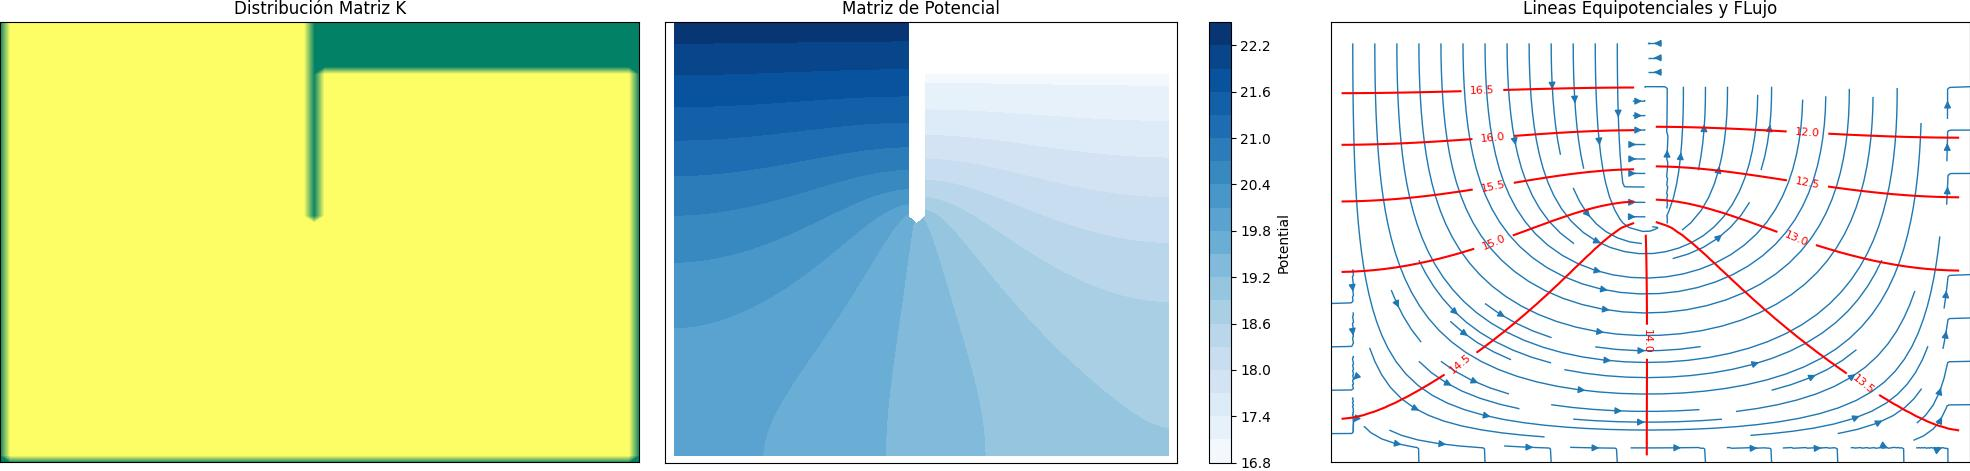
\includegraphics[width=1\textwidth]{GRAFICOS/laplace_caso_3.jpg}
    \caption{Gráfico de la función $f(x) = x^2$}
    \label{fig:caso_3}
\end{figure}

Se alcanzo la convergencia en la \textbf{iteracion 24670}
\\ \\
La velocidad de salida obtenida fue de \textbf{8.01e-05} m/s

\subsection{Caso Ejemplo Libro}

\begin{figure}[H]
    \centering
    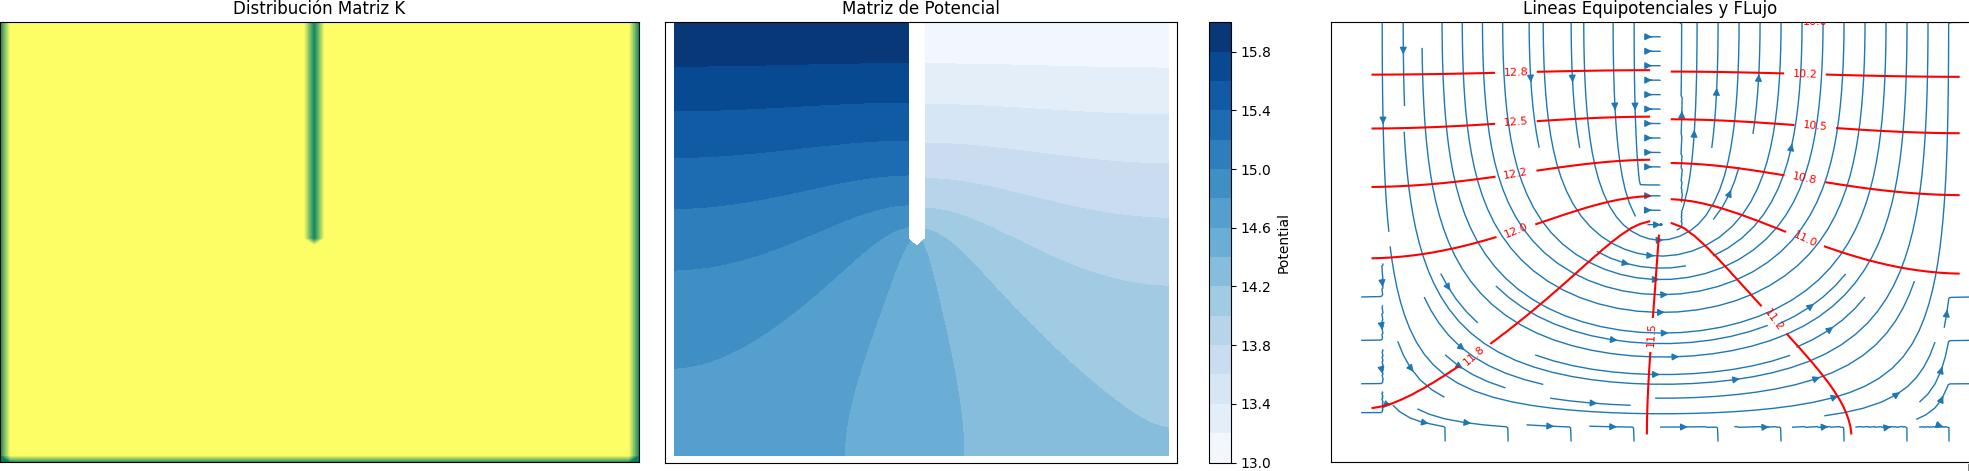
\includegraphics[width=1\textwidth]{GRAFICOS/laplace_caso_ejemplo.jpg}
    \caption{Gráfico de la función $f(x) = x^2$}
    \label{fig:caso_ejemplo}
\end{figure}

Se alcanzo la convergencia en la \textbf{iteracion 28172}
\\ \\
La velocidad de salida obtenida fue de \textbf{3.25e-06} m/s, de esta manera se corrobora que el codigo esta correctamente calibrado, ya que el resultado expuesto por el libro es de \textbf{3.2e-06} m/s.
\\ \\
Ademas, se realiza un caso doble, para ver como afecta la condicion de impermeabilidad de la barrera derecha en el flujo:

\begin{figure}[H]
    \centering
    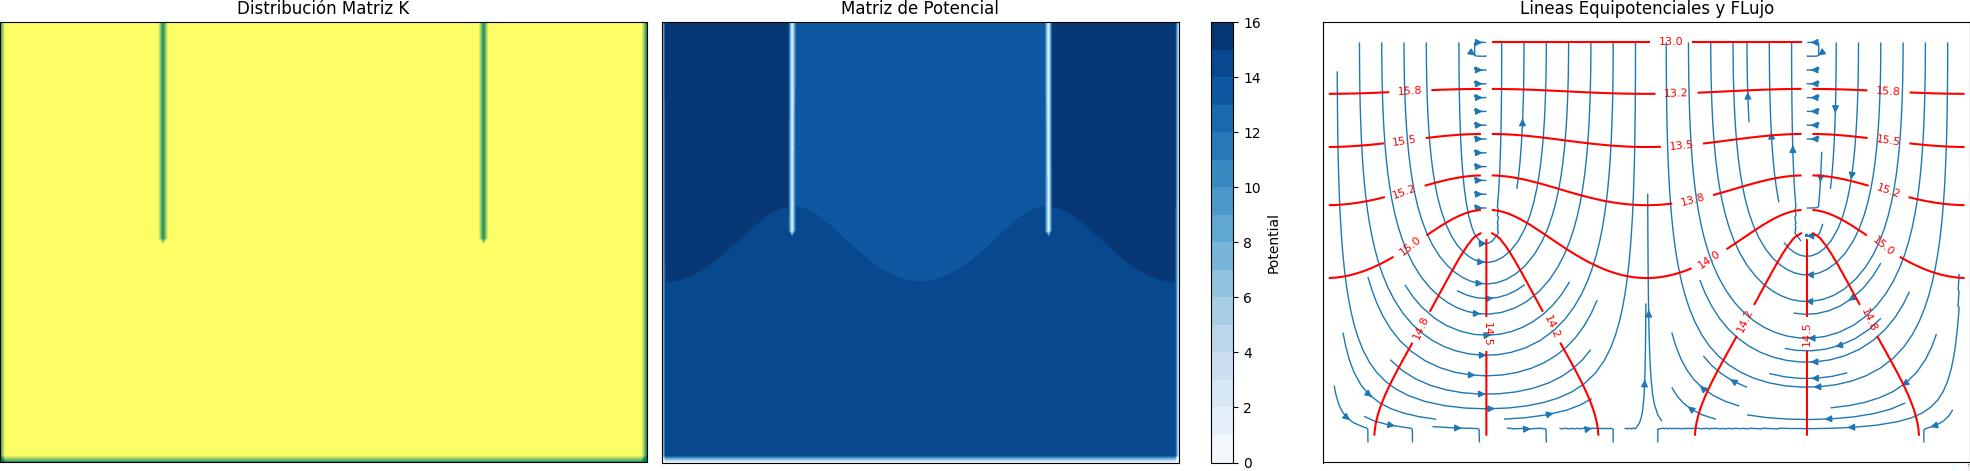
\includegraphics[width=1\textwidth]{GRAFICOS/laplace_caso_ejemplo_doble.jpg}
    \caption{Gráfico de la función $f(x) = x^2$}
    \label{fig:caso_ejemplo}
\end{figure}

Se alcanzo la convergencia en la \textbf{iteracion 16708}
\\ \\
La velocidad de salida obtenida fue de \textbf{2.63e-06} m/s.